\documentclass[a4paper,12pt,twoside]{article}
\usepackage[spanish]{babel}
\usepackage[utf8]{inputenc}
\usepackage{graphicx} %para insertar graficos/imagenes
\usepackage{amsmath} %para escribir matrices
\usepackage{amsfonts} %para poner \mathbb
\usepackage{float} %me deja usar la H de 'here' en los graficos para ponerlos donde yo quiera
\usepackage{anysize} %me permite definir los margenes como quiera
\usepackage{multirow} %para tablas con multicolumna
\usepackage{fancyhdr} % activamos el paquete
\usepackage{dcolumn}
\usepackage{multirow}

\usepackage{fixme}
\fxsetup{
    status=draft,
    author= carballeda ignacio,
    layout=inline, % also try footnote or pdfnote
}

\newcommand{\grad}{$^\circ$}

\newcommand{\codigoMateria}{66.10}
\newcommand{\nombreMateria}{Circuitos Electrónicos II}
\newcommand{\nroTP}{1}
\newcommand{\descripcionTP}{Informe de Avance del Proyecto}
\newcommand{\tituloTP}{Amplificador Clase G}
\newcommand{\facultad}{Facultad de Ingeniería}
\newcommand{\universidad}{Universidad de Buenos Aires}
\newcommand{\docentes}{José Alberto Bertuccio\\Federico D'Angiolo}

\pagestyle{fancy} % seleccionamos un estilo
\fancyhead{}
\fancyfoot{}
\lhead{\nombreMateria \, (\codigoMateria)} % texto izquierda de la cabecera
\rhead{\facultad} % texto centro de la cabecera
\cfoot{\thepage}

\marginsize{2cm}{2cm}{1cm}{1.5cm} %izquierda, derecha, arriba, abajo

\newcommand{\Direcrotio}{./}
\newcommand{\HRule}{\rule{\linewidth}{1mm}}


% Símbolos de las unidades
% Se utiliza el comando \ensuremath{~} por seguridad
% Incluyo también gensymb que añade los comandos:
%\degree, \celsius, \perthousand, \micro and \ohm
%	º		ºC			o/oo		µ			Ω

\usepackage{gensymb}

% VOLT
\newcommand{\nV}{\ensuremath{~\mathrm{nV}}}
\newcommand{\uV}{\ensuremath{~\mu\mathrm{V}}}
\newcommand{\mV}{\ensuremath{~\mathrm{mV}}}
\newcommand{\volt}{\ensuremath{~\mathrm{V}}}

% HERTZ
\newcommand{\hz}{\ensuremath{~\mathrm{Hz}}}
\newcommand{\hertz}{\ensuremath{~\mathrm{Hz}}}
\newcommand{\Hz}{\ensuremath{~\mathrm{Hz}}}
\newcommand{\khz}{\ensuremath{~\mathrm{kHz}}}
\newcommand{\kHz}{\ensuremath{~\mathrm{kHz}}}
\newcommand{\Mhz}{\ensuremath{~\mathrm{MHz}}}
\newcommand{\MHz}{\ensuremath{~\mathrm{MHz}}}

% FARAD
\newcommand{\pF}{\ensuremath{~\mathrm{pF}}}
\newcommand{\nF}{\ensuremath{~\mathrm{nF}}}
\newcommand{\uF}{\ensuremath{~\mu\mathrm{F}}}
\newcommand{\mF}{\ensuremath{~\mathrm{mF}}}
\newcommand{\farad}{\ensuremath{~\mathrm{F}}}

% OHM
%\newcommand{\ohm}{\ensuremath{~\Omega}}
\newcommand{\nohm}{\ensuremath{~\mathrm{n}\ohm}}
\newcommand{\uohm}{\ensuremath{~\mu\ohm}}
\newcommand{\mohm}{\ensuremath{~\mathrm{m}\ohm}}
\newcommand{\kohm}{\ensuremath{~\mathrm{k}\ohm}}
\newcommand{\Mohm}{\ensuremath{~\mathrm{M}\ohm}}

% HENRY
\newcommand{\uHy}{\ensuremath{~\mu\mathrm{Hy}}}
\newcommand{\nHy}{\ensuremath{~\mathrm{nHy}}}
\newcommand{\mHy}{\ensuremath{~\mathrm{mHy}}}
\newcommand{\henry}{\ensuremath{~\mathrm{Hy}}}

% AMPERE
\newcommand{\fA}{\ensuremath{~\mathrm{fA}}}
\newcommand{\uA}{\ensuremath{~\mu\mathrm{A}}}
\newcommand{\nA}{\ensuremath{~\mathrm{nA}}}
\newcommand{\mA}{\ensuremath{~\mathrm{mA}}}
\newcommand{\amper}{\ensuremath{~\mathrm{A}}}

% SEGUNDOS
\newcommand{\nS}{\ensuremath{~\mathrm{ns}}}
\newcommand{\uS}{\ensuremath{~\mu\mathrm{s}}}
\newcommand{\mS}{\ensuremath{~\mathrm{ms}}}
\newcommand{\seg}{\ensuremath{~\mathrm{s}}}

% WATTS
\newcommand{\mW}{\ensuremath{~\mathrm{mW}}}
\newcommand{\watt}{\ensuremath{~\mathrm{W}}}

% DECIBELES
\newcommand{\dB}{\ensuremath{~\mathrm{dB}}}
\newcommand{\dBm}{\ensuremath{~\mathrm{dBm}}}

% señal
\newcommand{\vs}[1]{%
\ensuremath{~v_{\mathrm{#1}}}%
}
\newcommand{\is}[1]{%
\ensuremath{~i_{\mathrm{#1}}}%
}

% ctes
\newcommand{\VA}{\ensuremath{~\mathrm{V}_{\mathrm{A}}}}
\newcommand{\VT}{\ensuremath{~\mathrm{V}_{\mathrm{T}}}}
\newcommand{\Vth}{\ensuremath{~\mathrm{V}_{\mathrm{th}}}}
\newcommand{\VCC}{\ensuremath{~\mathrm{V}_{\mathrm{CC}}}}
\newcommand{\VBB}{\ensuremath{~\mathrm{V}_{\mathrm{BB}}}}
\newcommand{\VDD}{\ensuremath{~\mathrm{V}_{\mathrm{DD}}}}
\newcommand{\VGG}{\ensuremath{~\mathrm{V}_{\mathrm{GG}}}}
\newcommand{\VSS}{\ensuremath{~\mathrm{V}_{\mathrm{SS}}}}
\newcommand{\RB}{\ensuremath{~\mathrm{R}_{\mathrm{B}}}}
\newcommand{\RC}{\ensuremath{~\mathrm{R}_{\mathrm{C}}}}
\newcommand{\RE}{\ensuremath{~\mathrm{R}_{\mathrm{E}}}}
\newcommand{\RL}{\ensuremath{~\mathrm{R}_{\mathrm{L}}}}
\newcommand{\RG}{\ensuremath{~\mathrm{R}_{\mathrm{G}}}}
\newcommand{\RD}{\ensuremath{~\mathrm{R}_{\mathrm{D}}}}
\newcommand{\RS}{\ensuremath{~\mathrm{R}_{\mathrm{S}}}}
\newcommand{\Rs}{\ensuremath{~\mathrm{R}_{\mathrm{s}}}}
\newcommand{\R}[1]{%
\ensuremath{~\mathrm{R}_{\mathrm{#1}}}%
}
\newcommand{\I}[1]{%
\ensuremath{~\mathrm{I}_{\mathrm{#1}}}%
}
\newcommand{\V}[1]{%
\ensuremath{~\mathrm{V}_{\mathrm{#1}}}%
}
\newcommand{\Ip}[1]{%
\ensuremath{~\hat{\mathrm{I}}_{\mathrm{#1}}}%
}
\newcommand{\Vp}[1]{%
\ensuremath{~\hat{\mathrm{V}}_{\mathrm{#1}}}%
}
\newcommand{\ip}[1]{%
\ensuremath{~\hat{i}_{\mathrm{#1}}}%
}
\newcommand{\vp}[1]{%
\ensuremath{~\hat{v}_{\mathrm{#1}}}%
}
\newcommand{\A}[1]{%
\ensuremath{~\mathrm{A}_{\mathrm{#1}}}%
}
\newcommand{\nada}{\quad{}}


\newenvironment{items}{
\begin{itemize}
  \renewcommand{\labelitemi}{$\bullet$}
  \setlength{\itemsep}{3pt}
  \setlength{\parskip}{1pt}
  \setlength{\parsep}{1pt}
}{
\end{itemize}}



\begin{document}



\begin{titlepage}

\thispagestyle{empty}

\begin{center}


\includegraphics[scale=0.15]{fiuba}\\[0.1cm]
\textsc{\universidad}\\[0.2cm]
\large{\textsc{\facultad}}\\[0.2cm]

\end{center}

\vfill

\begin{center}
\underline{\Large{\nombreMateria\, (\codigoMateria)}}
\end{center}

\vfill
\begin{center}

\end{center}
\vfill

\begin{center}
\Huge{\textsc{ \tituloTP }}\\[.5cm]
	\begin{figure}[H]
		\centering
		%\includegraphics[width=.5\textwidth]{bessel}
	\end{figure}\HRule \\[0.1cm]
\Huge{\textbf{\descripcionTP}}\\[0.01cm]
\HRule\\[0.3cm]
\end{center}

\vfill



\begin{tabbing}
	FECHA: \today\\
\\
	INTEGRANTES:\hspace{-1cm}\=\+\hspace{1cm}\=\hspace{6cm}\=\\
		Gomez, Cristian	\>\>- \#89968\\
			\>\footnotesize{$<$crisgvenezia@gmail.com$>$}\\
		Pollitzer, Ivan Gustavo	\>\>- \#22922\\
			\>\footnotesize{$<$igpollitzer@gmail.com$>$}\\
		Carballeda, Ignacio	\>\>- \#91646\\
			\>\footnotesize{$<$carballeda.ignacio@gmail.com$>$}\\

\end{tabbing}

\begin{flushleft} \large
\emph{Docentes:}\\[.2cm]
\end{flushleft}
\begin{tabbing}
\docentes\\[.5cm]
\end{tabbing}

\vfill

\hrule
\vspace{0.2cm}

\noindent\small{\codigoMateria\, --- \nombreMateria \hfill \facultad}

\end{titlepage}


\newpage
\vfill
\tableofcontents
\vfill

\newpage

\section{Actividades desarrolladas}

\subsection{Diseño conceptual}

Un amplificador consta, basicamente, de 3 etapas: una de entrada, diferencial, una intermedia, de ganancia de tensión, y una de salida, de ganancia de corriente.

Para la etapa de entrada, inicialmente consideramos una típica topografía diferencial, de colectores acoplados. Como los transistores no son componentes lineales, propusimos agregar otro par diferencial, en paralelo, con componentes complementarios; es decir, donde originalmente usamos transistores NPN, colocamos PNP, y viceversa.


Luego, conseguimos un circuito integrado, especialmente diseñado para audio, que presenta una distorsión considerablemente baja, por lo que decidimos usar este último.

Para la etapa intermedia, en primera instancia, decidimos utilizar un amplificador de 2 etapas, colector común - emisor común, con la diferencia del diseño convencional, de que la salida del VAS está conectada al centro del multiplicador de $V_{be}$, para obtener una mayor simetría en la última etapa.

Con el cambio a 2 pares diferenciales, la etapa intermedia también se duplica, complementariamente, y se conectan a la etapa de salida, por arriba y por abajo del multiplicador de $V_{be}$.

La etapa de salida es clase G, con transistores en configuración Darlington, para tener una ganancia de corriente elevada, y con transistores en paralelo, en la parte de mayor potencia, para repartir la corriente y disminuir la disipación de potencia en cada uno.

\subsection{Diseño circuital}

\begin{figure}[H]
\centering
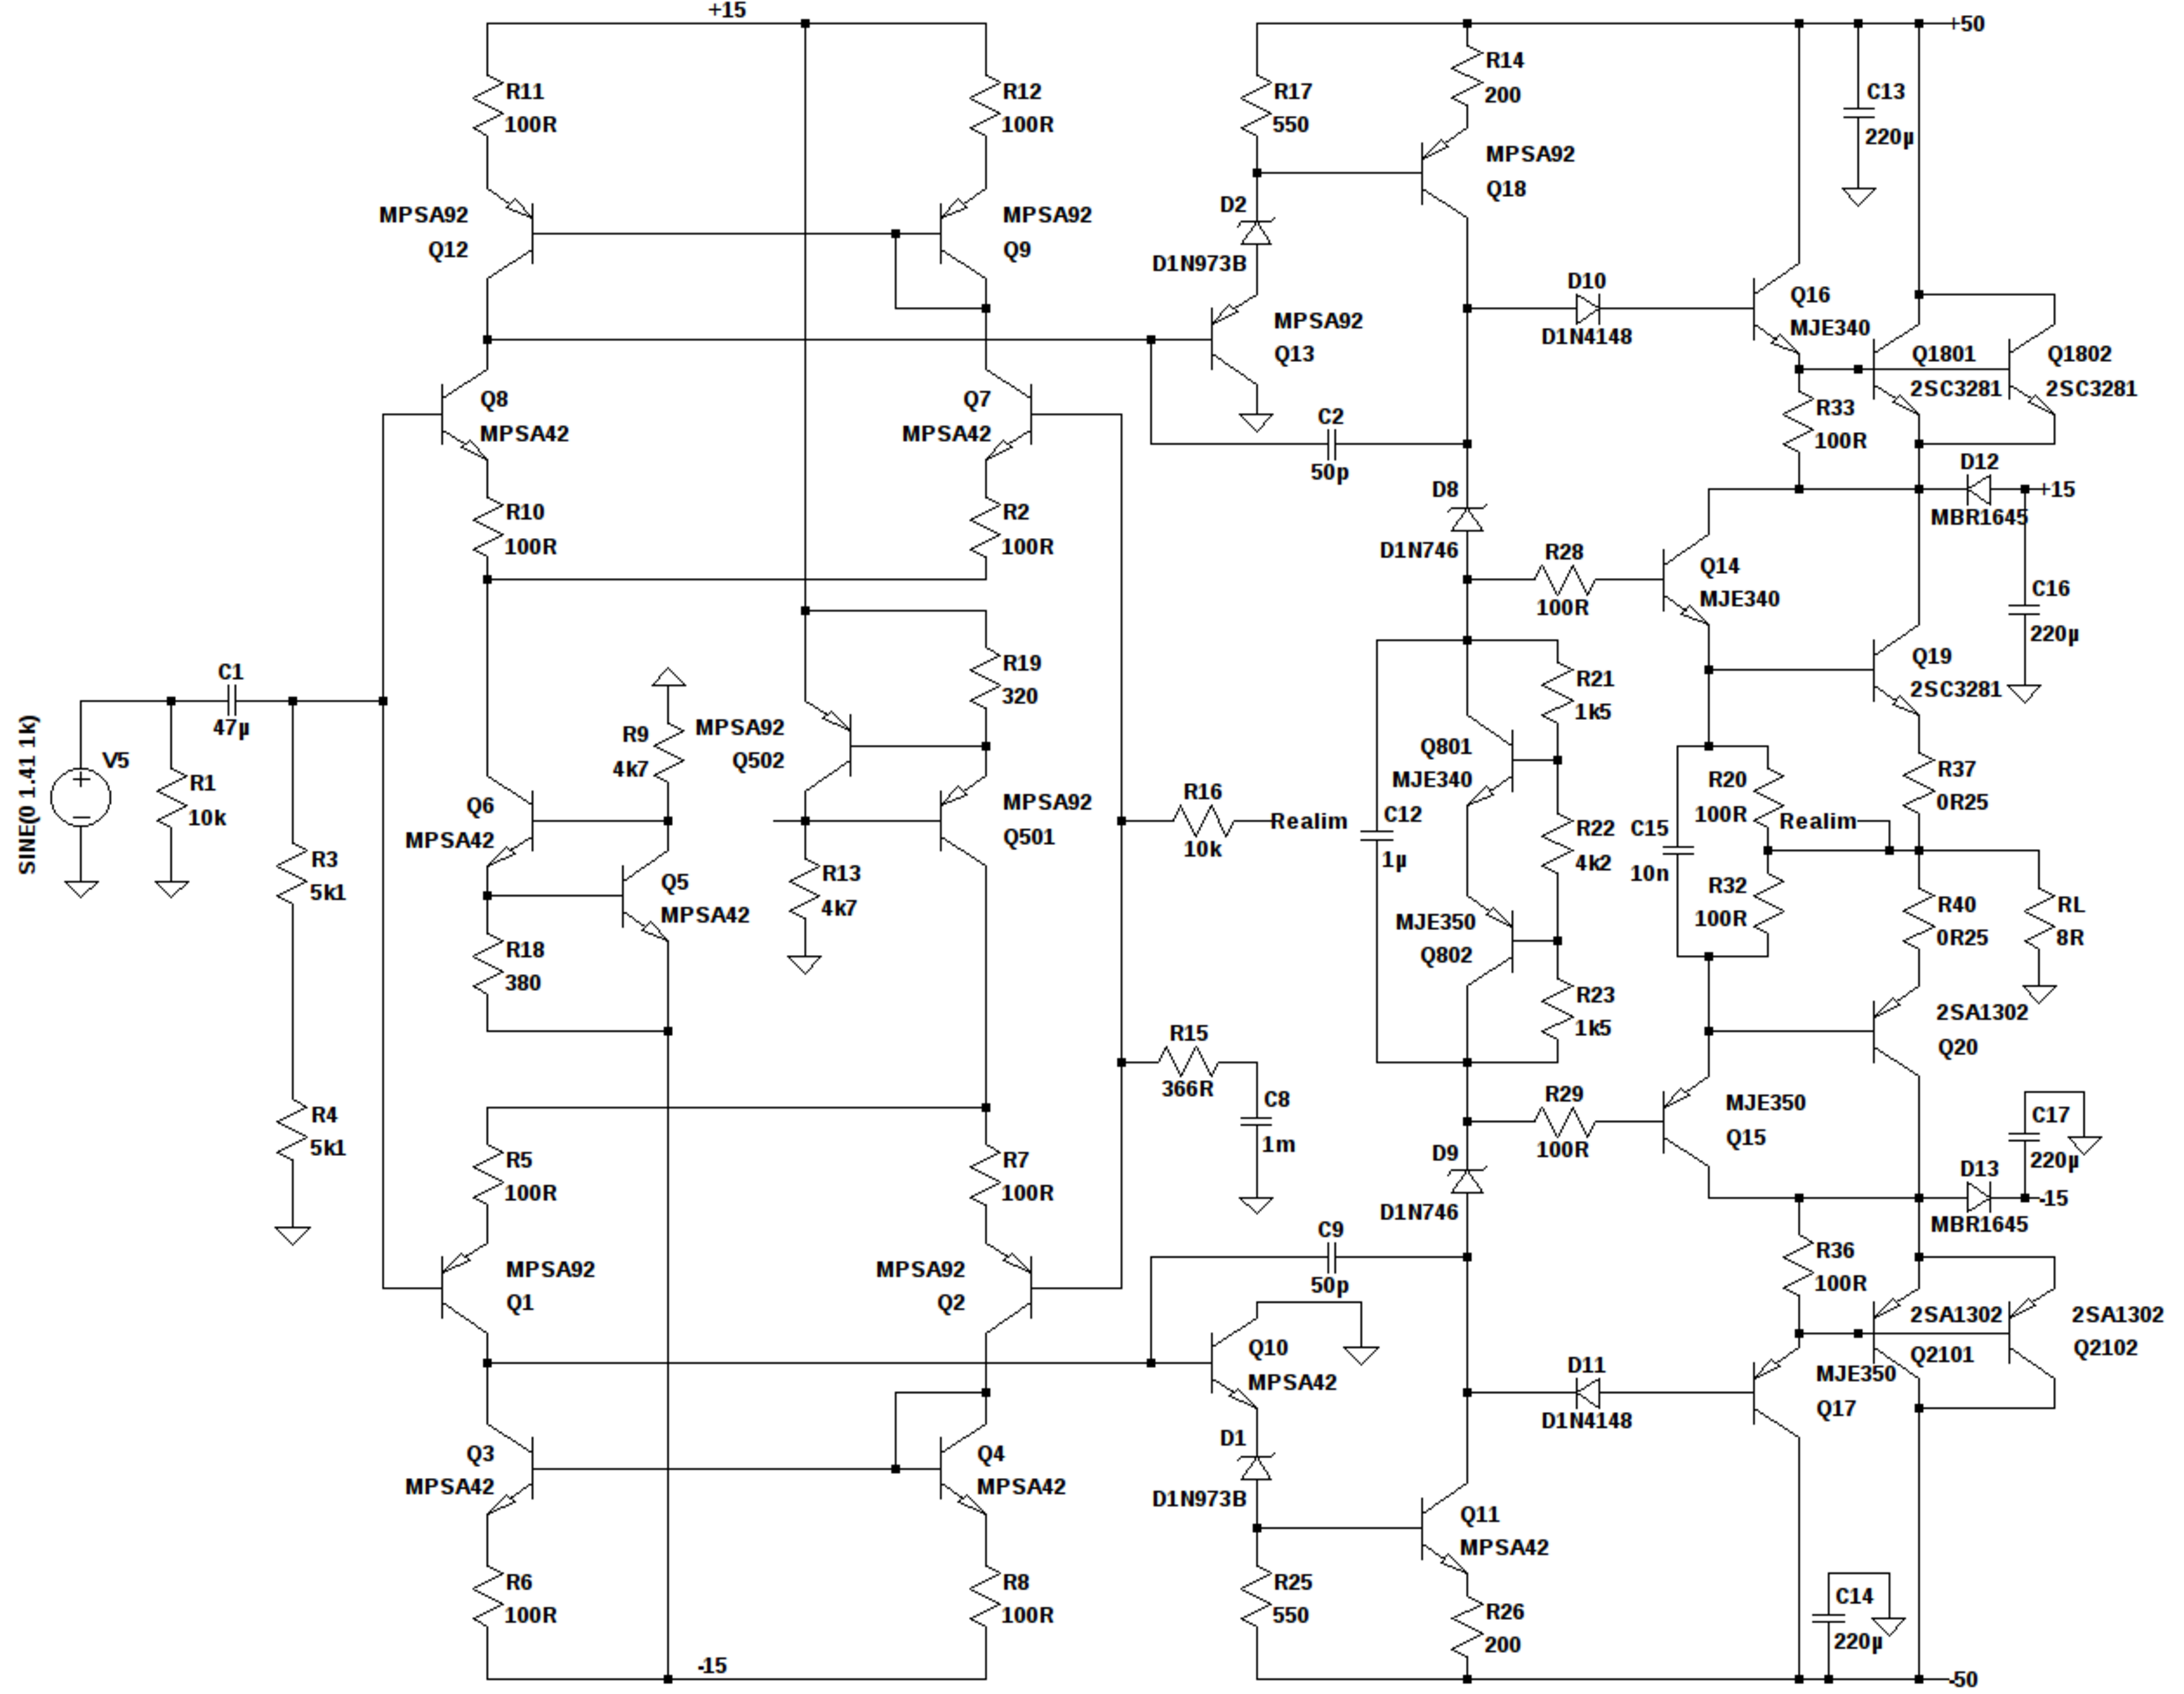
\includegraphics[scale=0.3]{img/circuito.pdf}
\caption{Circuito Diseñado}
\label{circuito} 
\end{figure}

\subsection{Análisis de los condicionantes de integración}



\subsection{Diseño PCB}


\section{Grado de avance}

Hasta el momento, hemos elegido las configuraciones de las distintas etapas, buscando aquellas que nos provean una menor distorsión; realizamos los cálculos para hallar los valores de realimentación, resistencias para el embalamiento térmico y los disipadores para los transistores; realizamos la simulación del circuito, y estamos en proceso de diseño de la fuente para reducir la tensión de alimentación a un valor apropiado para los integrados que utilizaremos en la primera etapa. 

\section{Dificultades encontradas}

Para el desarrollo del proyecto, nos encontramos con varios obstáculos. En el primer diseño que realizamos, nos encontramos con una disparidad en las corrientes del par diferencial, que resolvimos comprando transistores de más, midiendo sus parámetros $\beta$, y agrupándolos para poder trabajar con valores apareados. Otra solución que encontramos, y que aplicaremos en esta versión del circuito, es utilizar transistores integrados, que asegura que todos los transistores tengan las mismas propiedades, y estén apareados.


\section{Resumen de actividades a desarrollar}

Habiendo establecido todo lo anterior, procederemos con la simulación del circuito con las fuentes switching en la parte diferencial, el diseño del PCB comparte parte con la versión que realizamos el cuatrimestre pasado, por lo que sólo será necesario rediseñar la primera parte. Luego procederemos con el armado del circuito, verificando el correcto funcionamiento de las etapas, durante el armado de la placa, y luego tendremos que revisar que esté andando correctamente, y que cumpla con las parámetros que propusimos. Finalizado esto, procederemos a realizar las mediciones pertinentes.


\section{Dudas, cosas pendientes, blabla (ESTO NO VA)}

\begin{itemize}
\item No más de 10 páginas. Eso nos da excusas para no poner mucho, pero no nos da excusa para poner menos de 8. Jaja. Si nos nquedamos cortos, rellenemos hasta 10 y pongamos de excusa que no queríamos pasarnos para justificar lo que no hagamos
\item Cuentas en la sección de diseño circuital que nos hayan permitido elegir valores de componentes (??)
\item Pasar todo lo pasable del informe anterior a este. X ej, en diseño de PCB
\item Condicionantes de integración: preguntar mejor. Parece ser el asunto de disipación, acoplamiente térmico, masas locas en loop, ruteo, o lo que tenga que ver con pasar de la simulación con componentes ideales a la real. Capaz se pueden chupar un poco las medias de Fede chamullando algo sobre la clase que dio de ruido, y la importancia de la primera etapa.

\end{itemize}

\end{document}